%!TEX TS-program = xelatex
%!TEX encoding = UTF-8 Unicode

\documentclass[11pt]{extarticle}
% extarticle is like article but can handle 8pt, 9pt, 10pt, 11pt, 12pt, 14pt, 17pt, and 20pt text

\def \ititle {Joint Action and the Emergence of Mindreading}
\def \isubtitle {}
\def \iauthor {Stephen A. Butterfill}
\def \iemail{s.butterfill@warwick.ac.uk}
\date{}

%remove all section numbers
 \setcounter{secnumdepth}{0}

%for strikethrough
\usepackage[normalem]{ulem}

\input{$HOME/Documents/submissions/preamble_steve_handout}

\bibpunct{}{}{,}{s}{}{,}  %use superscript TICS style bib
%remove hanging indent for TICS style bib
%TODO doesnt work
\setlength{\bibhang}{0em}
%\setlength{\bibsep}{0.5em}


%itemize bullet should be dash
\renewcommand{\labelitemi}{$-$}

\begin{document}

\begin{multicols}{3}

\setlength\footnotesep{1em}


\bibliographystyle{newapa} %apalike

%\maketitle
%\tableofcontents



\

\begin{center}
{
\Large{Interacting Mindreaders}
}


%Stephen A. Butterfill

<butterfillS@ceu.hu>

\end{center}

Could interacting mindreaders be in a position to know things which they would be unable to know if they were manifestly passive observers? 



\section{Terminology}
\emph{Mindreading}: `In saying that an individual has a theory of mind, we mean that the individual imputes mental states to himself and to others ... the system can be used to make predictions, specifically about ... behavior.'\citep{premack_does_1978} %(Premack & Woodruff 1978: 515)

\emph{Sophisticated forms of mindreading} involve imputing propositional attitudes such as belief, desire and intention in the course of constructing or evaluating  reason-giving, causal explanations of action.

%\section{Joint action}
%Paradigm cases in philosophy include two people 
%	painting a house together, \citep{Bratman:1992mi}
%	lifting a heavy sofa together, \citep{Velleman:1997oo} 
%	preparing a hollandaise sauce together, \citep{Searle:1990em}
%	going to Chicago together, \citep{Kutz:2000si} 
%	and walking together. \citep{gilbert_walking_1990}
%
%In developmental psychology paradigm cases of joint action include  two people 
%	tidying up the toys together, \citep{Behne:2005qh}
%	cooperatively pulling handles in sequence to make a dog-puppet sing, \citep{Brownell:2006gu} 
%	and bouncing a block on a large trampoline together.\citep{Tomasello:2007gl}
%
%Other paradigm cases from research in cognitive psychology include two people
%	lifting a two-handled basket,  \citep{Knoblich:2008hy}
%	putting a stick through a ring, \citep{ramenzoni_joint_2011}
%	and swinging their legs in phase.\citep%[p. 284]
%	{schmidt_richardons:_2008}


\section{The Problem of Opaque Means}
Ignorance about to which ends actions are means can be an obstacle to goal ascription.

\section{Distributive Goals}
A \emph{goal} is an outcome to which actions are, or might be, directed.  A \emph{goal-state} is an intention or other state of an agent linking an action to a goal to which it is directed.

%A \emph{goal-directed joint action} is a joint action which, taken as a whole, is directed to a goal.

The \emph{distributive goal} of two or more actions is G: (a) each action is individually directed to G; and (b) it is possible that: all actions succeed relative to this outcome.

%\textbf{Collective goal}.  The \emph{collective goal} of two or more actions is G:
%(a) G is a distributive goal of the outcomes;
%(b) the actions are coordinated; and 
%(c) coordination of this type would normally  facilitate occurrences of outcomes of G's type



\section{Ordinary 3$^{\textrm{\tiny rd}}$ person interpretation} 

Csibra \& Gergely's principle of rational action: `an action can be explained by a goal state if, and only if, it is seen as the most justifiable action towards that goal state that is available within the constraints of reality.'\citep{Csibra:1998cx,Csibra:2003jv}

(Contrast a principle of efficiency:
`goal attribution requires that agents expend the least possible amount of energy within their motor constraints to achieve a certain end.' \citep%[p.\ 1061]
{Southgate:2008el})

%



These facts:
%
\begin{enumerate}
%
\item action $a$ is directed to some goal;
%
\item actions of $a$'s type are normally capable of being means of realising outcomes of $G$'s type in situations with the salient (to any concerned) features of this situation;
% 
\item no alternative type of action is both 
typically available to agents of this type 
and also 
such that actions of this type would be normally be significantly better* means of realising outcome $G$ in situations with the salient features of this situation;
%
\item the occurrence of outcome $G$ is typically desirable for agents of this type;
%
\end{enumerate}
%
\begin{enumerate}[resume]
\item there is no other outcome, $G'$, 
the occurrence of which would be at least comparably desirable for agents of this type 
and where (2) and (3) both hold of $G'$ and $a$
%
%where
%	the occurrence of $G'$ would be at least comparably desirable for agents of this type 
%%where
%%	$G$'s occurrence is not a means to $G'$'s nor conversely,
%and
%where  
%	(2) and (3) both hold of $G'$ and $a$
\end{enumerate}
%
may jointly constitute defeasible evidence for the conclusion that:
%
\begin{enumerate}[resume]
\item $G$ is a goal to which action $a$ is directed.
\end{enumerate}
%

{
\footnotesize
*An action of type $a'$ is a better means of realising outcome $G$ in a given situation than an action of type $a$ if, for instance, actions of type $a'$ normally involve less effort than actions of type $a$ 
in situations with the salient features of this situation 
and everything else is equal; 
or if, for example, actions of type $a'$ are normally more likely to realise outcome $G$ than actions of type $a$
in situations with the salient features of this situation 
and everything else is equal.
}

%\section{The problem of opaque means}
%Ordinary 3$^{\textrm{\tiny rd}}$ person interpretation may fail when it is not known which outcomes a behaviour is a means of bringing about, especially where a novel tool or communicative device is used.

\section{Your-goal-is-my-goal}
\begin{enumerate}
\item You are willing to engage in some joint action or other with me.
%(for example, because you have made eye contact with me while I was in the middle of attempting to do something).

\item I am not about to change the single goal to which my actions will be directed.

\end{enumerate}
%
Therefore:
%
\begin{enumerate}[resume]
%
\item A goal of your actions will be my goal, the goal I now envisage that my actions will be directed to.
\end{enumerate}
%

\section{Application}

`to understand pointing, the subject needs to understand more than the individual goal-directed behaviour. She needs to understand that ... the other attempts to communicate to her ...  and ... the communicative intention behind the gesture'\citep{Moll:2007gu}


\begin{center}
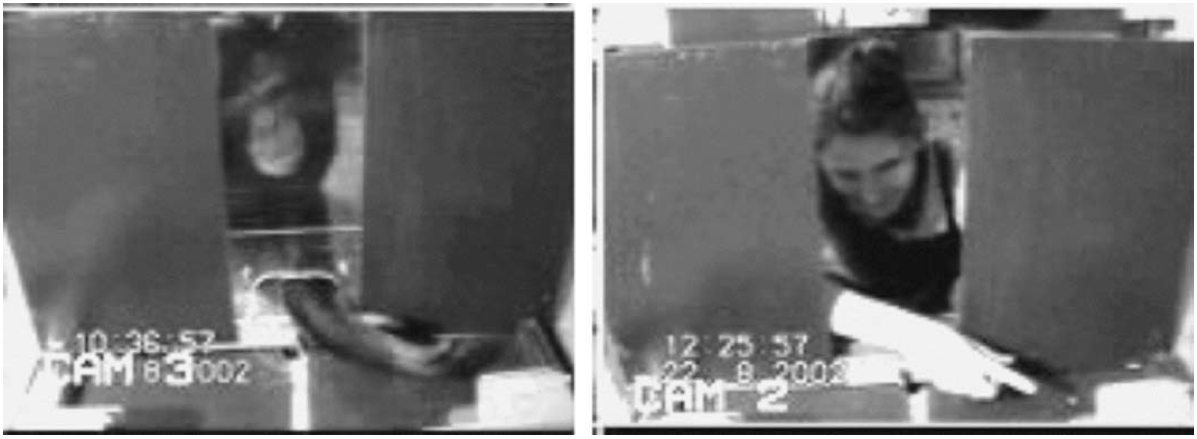
\includegraphics[width=6cm]{figure_hare_toma_2004_e3.png}
\label{fig:reach_point}

A failed reach (left) and a helpful point (right).\citep%[p.\ 557, figure 4]
	{hare_chimpanzees_2004}
\end{center}



Leekam et al.: `the adult’s social cues conveyed her communicative intent, which in turn encouraged the child to `see through the sign'.'
\citep%[p.\ 118]
{leekam_adults_2010}


Csibra: Early in human development,
teleological and referential action interpretation 
`rely on different kinds of action understanding' %\citep[p.\ 456]{Csibra:2003kp}
and
involve two distinct `action interpretation systems'   %\citep[p.\ 456]{Csibra:2003kp} 
which come together later in development.\citep{Csibra:2003kp}



\footnotesize 
\bibliography{$HOME/endnote/phd_biblio}

\end{multicols}

\end{document}